\DailyTitle{6364 Log (November 18, 2010)}

\DailySection{Summary List}

\begin{enumerate}
\item Looked at timing filter performance
\item Had a presentation in the noise WG meeting
   \begin{enumerate}
   \item Look at 50ns run.
   \item Test time performance on \texttt{MultiJet} dataset
   \end{enumerate}
\end{enumerate}

\DailySection{Timing filter}

The filter is taken from
\url{http://cmssw.cvs.cern.ch/cgi-bin/cmssw.cgi/CMSSW/JetMETAnalysis/HcalReflagging/python/hbherechitreflaggerJETMET_cfi.py?hideattic=0&revision=1.5&view=markup&pathrev=V00-00-18}
updated by Phil.

Timing is already good if the global tag used is recent enough.

A couple performance plots are shown in figures \ref{Figure_6364_TimingHBHEMET} and \ref{Figure_6364_CleanedPercentageWithTiming}.
Note that at 50 GeV, the cleaning efficiency is roughly 88\%.  Timing cut successfully picked out a lot of the remaining noises.
There might not be a need for round 3 variables.  Let's take a look at the rest in any case.
Maybe there is something obvious to cut on.

\begin{figure}
   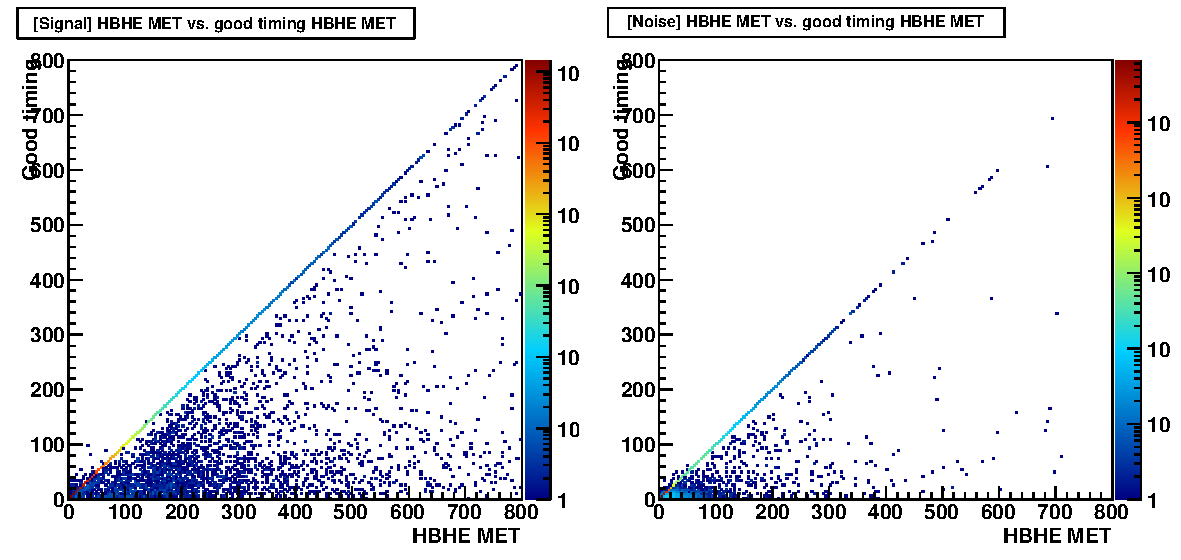
\includegraphics[width=120mm]{DailyLog/6364/6364_Comparison10_Comparison_HHBHEMETVsGoodTimingHBHEMET}
   \caption{HBHEMET before and after timing cut}
   \label{Figure_6364_TimingHBHEMET}
\end{figure}

\begin{figure}
   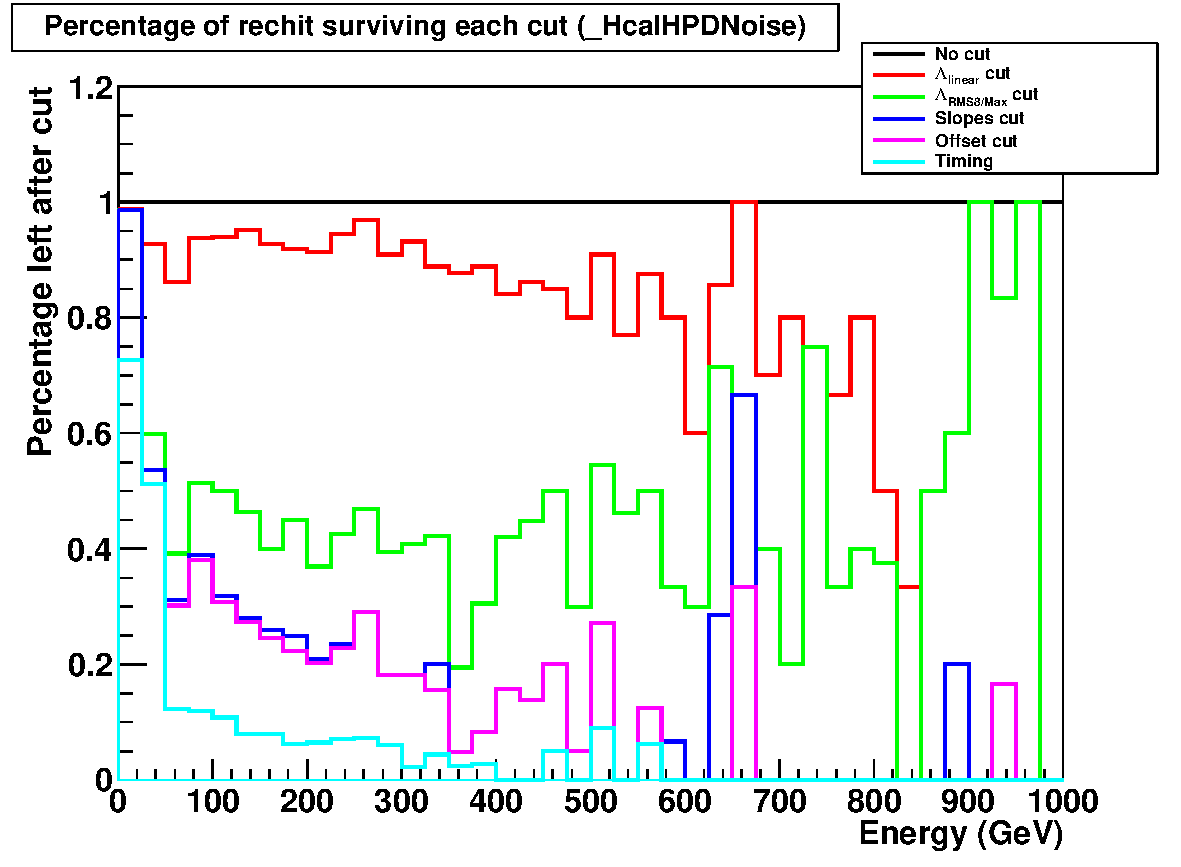
\includegraphics[width=120mm]{DailyLog/6364/6364_RecHitEnergyRatioPlot_HcalHPDNoise}
   \caption{Percentage of pulses remaining after each step of cut, including timing filter}
   \label{Figure_6364_CleanedPercentageWithTiming}
\end{figure}


